%!TEX root = ../documentation.tex

\chapter{Application requirement analysis}\label{cha:requirement}

In order to evaluate if there is a need for a generalized shell application, it is important to first understand what the requirements for such an application are.
To get the needed insights a requirement analysis is conducted via literature research and the expert interviews.
This chapter focuses on outlining requirements and comparing them against each other.

The found requirements can be divided into categories.
These are explained in section \ref{cha:requirement_categories}.
After that, an overview of all requirements is provided in the section \ref{cha:requirements_overview}.
This includes an explanation on how the requirements were compared against each other in terms of importance, and an overview, seen in Table \ref{tbl:overview_requirements}, which contains all found requirements.
Following that are multiple sections which describe the requirements in detail (section \ref{cha:requirement_detail_integration}, \ref{cha:requirement_detail_performance}, \ref{cha:requirement_detail_state}, \ref{cha:requirement_detail_style} and \ref{cha:requirement_detail_developer}).
Lastly, a conclusion for this chapter is drawn in section \ref{cha:requirements_conclusion}.



%!TEX root = ../../documentation.tex

\section{Requirement categories}\label{cha:requirement_categories}

During the requirements research it became apparent that requirements can be divided into categories.
Grouping requirements by categories further structures the analysis.
This also allows to order them based on there importance.
Thus, the following list shows an interpretation of requirement categories and their importance in descending order.
Each category is abbreviated, except \textit{Performance}, as seen in the following list.
They are also used in the Table \ref{tbl:overview_requirements}.

\pagebreak

\begin{enumerate}
    \item Browser routing and integration approach \textit{(Integration)}
    \item Performance
    \item Shared state and micro frontend inter-communication techniques \textit{(State)}
          \begin{itemize}
              \item Internationalization
              \item Authentication
          \end{itemize}
    \item Styling handling \textit{(Style)}
    \item Developer experience \textit{(Developer)}
          \begin{itemize}
              \item Tools
              \item Debugging
              \item Testing
          \end{itemize}
\end{enumerate}

To challenge the interpretation, each expert was asked to validate it.
This was the third question of the expert interviews (see Appendix \ref{cha:appendix_expertinterview_questions}).
All experts agreed with the selected categories, but the order of importance was slightly different.
An overview of all opinions about the importance is shown in Table \ref{tbl:overview_requirements_categories}.
The number on the left indicates the score.

\begin{table}[h]
    \setlength{\tabcolsep}{4.265pt} % Default value: 6pt
    \begin{tabularx}{\linewidth}{|l|l|l|l|l|l|l|}
        \hline
        \textbf{S}                              &
        \textbf{LM} \cite{Vogel.2020.Mezzalira} &
        \textbf{PR} \cite{Vogel.2020.Rehm}      &
        \textbf{PH} \cite{Vogel.2020.Huber}     &
        \textbf{MS} \cite{Vogel.2020.Steyer}    &
        \textbf{BO} \cite{Vogel.2020.Olleck}    &
        \textbf{IJ} \cite{Vogel.2020.Jovanovic}
        \\ \hline
        1
                                                &
        Integration
                                                &
        Integration
                                                &
        Integration
                                                &
        Integration
                                                &
        Integration
                                                &
        Performance
        \\ \hline
        2
                                                &
        State
                                                &
        Performance
                                                &
        State
                                                &
        Performance
                                                &
        State
                                                &
        Integration
        \\ \hline
        3
                                                &
        Developer
                                                &
        State
                                                &
        Performance
                                                &
        State
                                                &
        Performance
                                                &
        State
        \\ \hline
        4
                                                &
        Performance
                                                &
        Style
                                                &
        Style
                                                &
        Style
                                                &
        Style
                                                &
        Style
        \\ \hline
        5
                                                &
        Style
                                                &
        Developer
                                                &
        Developer
                                                &
        Developer
                                                &
        Developer
                                                &
        Developer
        \\ \hline
    \end{tabularx}
    \caption{Overview of the different opinions about requirement categories}
    \label{tbl:overview_requirements_categories}
\end{table}

% score calculation explanation
In order to determine the order of importance based on the expert's opinion, a score is calculated.
Each position is weighted with a number equal to the order, which is the first column \textit{S}.
The most important is equal to 1, the second is equal to 2 and so on.
The final score of each category is determined by averaging all scores.
The results are shown in Table \ref{tbl:category_scores}.
In conclusion, \textit{Integration} is the most important category.
Following that is the \textit{Performance} and \textit{State} on second, followed by \textit{Style} and lastly \textit{Developer}.
The result is close to the initially predicted order of importance.

\begin{table}[h]
    \newcolumntype{s}[1]{>{\hsize=#1\hsize}X}
    \begin{tabularx}{\linewidth}{|X|X|X|X|X|}
        \hline
        \textbf{Integration} &
        \textbf{Performance} &
        \textbf{State}       &
        \textbf{Style}       &
        \textbf{Developer}
        \\ \hline
        $ \approx 1,2$
                             &
        $ \approx 2,5$
                             &
        $ \approx 2,5$
                             &
        $ \approx 4,2$
                             &
        $ \approx 4,7$
        \\ \hline
    \end{tabularx}
    \caption{Requirement categories scores based on expert opinions}
    \label{tbl:category_scores}
\end{table}


\section{Requirement analysis result overview}\label{cha:requirements_overview}

The analysis led to many requirements.
To better outline the importance of each requirement, they need to be scored in some way.
In order to achieve this, the process of the pairwise comparison technique is used.
This technique determines the relative importance by comparing requirements against each other and thus, obtaining a score for all requirements \cite[p.~573]{Achimugu.2014}.

The technique was modified in order to use it for the requirement analysis.
Instead of weighting the requirements, the expert statements are weighted based on the questions.
In the expert interviews, the questions four, five and six are used to gain insights into requirements and their approaches (see \ref{cha:appendix_expertinterview_questions}).
Each of the questions is assigned with a different weight.

\begin{itemize}
    \item Question four, \textit{What are requirements for the named shell application scenario which you had from a customer?}: They can be an any importance and thus, receive a score of 1
    \item Question five, \textit{Can you name any requirements which are needed for all shell application scenarios?}: These are the most important requirements in context of this thesis and thus, receive a score of 3
    \item Question six, \textit{What are the most difficult requirements to achieve and why?}: A general goal of architecture is to reduce the complexity of a project \cite[p.~98]{AlSharif.2004} and therefore, these requirements receive a score of 2
\end{itemize}

By introducing the score the focus can be shifted towards the relevant requirements.
Therefore, the requirements with a score of 5 or higher are considered relevant.
The reason is, that a low score makes it less likely that a requirement is actually needed.
It is important to note, that not all requirements can be part of a generalized shell application.
Hence, low scoring requirements are considered but they are a optional feature of the generalized shell application.


The requirements analysis was not only conducted via the expert interview, but also through a literature research.
Requirements found in the literature research receive a score of 1, because the context is not the same as in the expert interviews and therefore, comparability is not guaranteed \cite[p.~35]{AlexanderBognerBeateLittigWolfgangMenz.2009}.
On the other hand, requirements mentioned in literature should be considered as well to ensure a broad view.
Therefore, a score equivalent of question four in the interview is suitable.

After collecting the weights for each requirement, the weights are added up and resulting in the score.
In case of a score tie, the respective requirements are considered equally relevant.
Also, requirements are not only ordered by their score, but also by their respective category.
The categories are explained in the next section \ref{cha:requirement_categories}.

An overview of the requirement analysis result is shown in Table \ref{tbl:overview_requirements}.
In addition to this Table, there are two more tables in the appendix \ref{cha:appendix_requirements_overview}.
The first (\ref{tbl:adx_requirements_scores}) shows the score of each requirement and the second (\ref{tbl:adx_requirements_references}) shows which reference mentioned the requirement, considers it as difficult and as critical.
Further detail for the requirements will be provided in the following sections from  \ref{cha:requirement_detail_integration} to \ref{cha:requirement_detail_developer}.

%!TEX root = ../../documentation.tex

\setlength{\tabcolsep}{4.265pt} % Default value: 6pt
\begin{longtable}{|l|l|p{0.56\textwidth}|}
	% \begin{longtable}{ l l p{0.56\textwidth} }
	\hline
	\textbf{Category}             & \textbf{Requirement}   & \textbf{Description}                                                                               \\ \hline
	\multirow{12}{*}{Integration} & Loading                & Load a \ac{MF} into the application and provide it for further use                                 \\ \cline{2-3}
	                              & Lifecycle management   & A \ac{MF} can be bound and unbound to the \ac{DOM}                                                 \\ \cline{2-3}
	                              & Routing                & Enable page changes based on the \ac{URL} changes                                                  \\ \cline{2-3}
	                              & Configuration          & Behavior of \ac{MF} should be configurable                                                         \\ \cline{2-3}
	                              & Integration            & Compose a \ac{MF} into the current application                                                     \\ \cline{2-3}
	                              & Shared logic           & The shell provides logic for all \ac{MF}                                                           \\ \cline{2-3}
	                              & Widgets                & A \ac{MF} exposes a widget which can be used by an other \ac{MF}                                   \\ \cline{2-3}
	                              & Page layout            & The shell should control the page layout                                                           \\ \cline{2-3}
	                              & Indexable via crawler  & The application needs to be indexable via crawler                                                  \\ \cline{2-3}
	                              & \ac{MF} interoperable  & A \ac{MF} should be able to run in multiple applications                                           \\ \cline{2-3}
	                              & Abstraction layer      & The shell should abstract browser \ac{API} calls which differ between platforms                    \\ \cline{2-3}
	                              & Third party extensible & Consumers should be able to extend the application with external UIs                               \\ \hline
	Performance                   & Performance            & Ensure that the application performs as expected                                                   \\ \hline
	\multirow{5}{*}{State}        & State exchange         & A \ac{MF} needs to know the application state to display content accordingly                       \\ \cline{2-3}
	                              & Intercommunication     & MFs need to interact with each other via some form of communication                                \\ \cline{2-3}
	                              & Security               & The application needs authentication and authorization                                             \\ \cline{2-3}
	                              & Internationalization   & The application should be able to change based on language and county                              \\ \cline{2-3}
	                              & Consistent style       & Ensure that the application has a consistent style                                                 \\ \hline
	\multirow{6}{*}{Developer}    & Autonomy               & Each \ac{MF} should be independent, which includes technology, development, testing and deployment \\ \cline{2-3}
	                              & Configuration          & Behavior of \ac{MF} should be configurable                                                         \\ \cline{2-3}
	                              & Experience             & Compensate the complexity of \ac{MFA} for the developers                                           \\ \cline{2-3}
	                              & Tools                  & Tools to support developers                                                                        \\ \cline{2-3}
	                              & Debugging              & Provide an approach for debugging a \ac{MF}                                                        \\ \cline{2-3}
	                              & Testing                & A \ac{MF} should be testable                                                                       \\ \hline

	\caption{Overview of requirements for a \ac{MF} application which are collected in the expert interviews and research}
	\label{tbl:overview_requirements}
\end{longtable}
\setlength{\tabcolsep}{\spaltenabstand}

%!TEX root = ../../documentation.tex

\section{Integration requirements and approaches}\label{cha:requirement_detail_integration}

This section explains the integration requirements.
The requirements from \textit{\nameref{cha:requirement_detail_integration_loading}} until \textit{\nameref{cha:requirement_detail_integration_sharedlogic}} are described in greater detail, than the requirements from \textit{\nameref{cha:requirement_detail_integration_widget}} to \textit{\nameref{cha:requirement_detail_integration_extensible}}, due to their score.





\subsection{Loading}\label{cha:requirement_detail_integration_loading}

The \textit{\nameref{cha:requirement_detail_integration_loading} (\textbf{Score 14})} requirement is about the shell's ability to load a \ac{MF} when needed.
Before describing the approaches, it is important to consider what data needs to be loaded.
A \ac{MF} consists of at least one \ac{JS} file.
Other files are for instance, \ac{CSS}, \ac{HTML}, \ac{JSON} and image files.
Depending on the \ac{MF} the number of files which need to be loaded may vary.
Therefore, the loading approach must be flexible.
End-users also expect the application to be fast \cite[p.~244p]{Zhou.2008}.
Thus, the number of files needed for running the \ac{MF} should be small.
Finally, the shell application needs to know which files need to be loaded.
This is further discussed in the \textit{\nameref{cha:requirement_detail_integration_configuration}} requirement.
There are two approaches on loading a \ac{MF} as well as an optional approaches that can be used on top.

The first approach uses the browser \ac{API} to load the files.
\textciteMezzalira{} proposes that one \ac{HTML} file per \ac{MF} is exposed and it contains all tags needed to load and startup the application.
A little \ac{JS} code is responsible to load the \ac{HTML} file and integrate all tags into the application.
The Browser then automatically starts downloading the needed files.
Another variant of this, which also utilizes the browser \ac{API}, is to add each loading tag individually in the current application.
This was mentioned by \textcite{Dornenburg.2019} and \textcite{Laug.2018}.

The second approach only addresses \ac{JS} files.
It uses \ac{JS} module import for loading the files.
As soon as the file is fully loaded, it is executed.
So, in this approach no tags are added to the current application and the \ac{JS} file is only loaded and executed within \ac{JS} \cite{Vogel.2020.Olleck}.
According to \citeauthorMezzalira{} it is quicker to let the browser load the files, than executing \ac{JS} upfront to load it.

Finally, on top of the named approaches a Service Worker can be used for caching and preloading, which was mentioned by \textciteRehm{} and \textciteSteyer{}.
Service Workers run in a separate thread from the \ac{UI} and can cache images, scripts, styles or even pages \cite[p.~24f.]{Sheppard.2017}.

This requirement has the highest score for the Integration category.
It is considered crucial from \textciteHuber{} and difficult from \textciteMezzalira{}, \textciteSteyer{}, \textciteOlleck{} and \textciteJovanovic{}.





\subsection{Lifecycle management}\label{cha:requirement_detail_integration_lifecycle}

The requirement \textit{\nameref{cha:requirement_detail_integration_lifecycle} (\textbf{Score 10})} is an extension to the \textit{\nameref{cha:requirement_detail_integration_integration}} requirement.
In general \textit{\nameref{cha:requirement_detail_integration_integration}} is about which technique is used to include a \ac{MF} into the application, the \textit{\nameref{cha:requirement_detail_integration_lifecycle}} is about the \acp{MF} visibility and loading state.
A \ac{MF} lifecycle can consist of multiple events which represent its current state.
These events could be triggered by the shell application or by the \ac{MF} itself.
\textciteOlleck{} named states he used in a project, which are \textit{bootstrap}, \textit{display}, \textit{hide} and \textit{destroy (or clear)}.
\textit{Bootstrap} represents the integration and startup, \textit{display} represents that a \ac{MF} is shown to the user, \textit{hide} is the opposite of display and \textit{destroy} or \textit{clear} represents that the \ac{MF} is unloaded and its occupied resources are free.
Note, that this is one example and not all applications need such an extensive lifecycle.
Another example from \textciteRehm{} provides only the \textit{bootstrap} event, which is raised when a \ac{MF} is in the integration process.
\citeauthorRehm{} and \textciteSteyer{} state that lifecycle management an optional feature.

For this requirement, no explicit approach is mentioned other than raising events and this is part of the \textit{\nameref{cha:requirement_detail_state_intercommunication}} requirement.
The only explicit description of a functionality is, that in case of a destroy or clear event the \ac{MF} must provide a function which is called to remove all event listener.
\textciteMezzalira{} points out, that in this case an interface which provides such a function is needed.
This requirements was mentioned as difficult from \textciteJovanovic{} and \citeauthorMezzalira{}, and as crucial from \textciteHuber{}.





\subsection{Routing}\label{cha:requirement_detail_integration_routing}

\textit{\nameref{cha:requirement_detail_integration_routing} (\textbf{Score 9})} is about
\ac{URL} changes that are reflected in the \ac{UI}.
Updating the \ac{UI} consists of either changing the current page layout or swapping \acp{MF} accordingly.
The idea of changing the page layout based on the route is further described in the \textit{\nameref{cha:requirement_detail_integration_pagelayout}} requirement.

There is an important first differentiation in terms of how the application functions.
The differentiation depends on the business domain size which each \ac{MF} covers.
But the important part for routing is, that a \ac{MF} either has only one page or multiple pages.
In the first case, only the shell needs routing functionality, while the latter is a combination of both.
No matter which approach is used, all experts mention splitting the \ac{URL} into different sections.
These sections have different responsibilities.
The base route of the \ac{URL} is mentioned in the following two examples.
It is the value between the first and second slash in the \ac{URL}.

\textcite{Grijzen.2019} provides an example where only the shell is responsible for routing.
No implementation details are shared, but his example is combined with the \textit{\nameref{cha:requirement_detail_integration_pagelayout}} requirement.
The base route determines which \ac{MF} is shown, while a query parameter\footnotemark  is added to save the page layout and distribution of other \acp{MF}.
\footnotetext{\url{https://developer.mozilla.org/en-US/docs/Web/API/URLSearchParams} (Visited on 09/06/2020)}

Another example provided by \textciteRehm{} and \textciteSteyer{} addresses the idea of splitting the routing responsibility between the shell and \acp{MF}.
In the example, the shell manages the base route.
Based on this value one \ac{MF} is shown and it is responsible for the rest of the \ac{URL}.
Therefore, it provides its own router that handles page changes which are within itself.
This results in a hierarchical setup, where the shell sits on top and is essentially a meta router between \acp{MF}, which in turn routes on their own.

\textciteSteyer{} points out, that there are some difficulties with this approach and it boils down to the fact, that the browser \ac{API} does not support an event for \enquote{\ac{URL} has changed}.
He goes on to say, that there is a workaround for this problem, which is monkey patching\footnotemark the browser to support such an event.
\footnotetext{\url{https://web.archive.org/web/20080604220320/http://plone.org/documentation/glossary/monkeypatch} (Visited on 09/06/2020)}
The only browser \ac{API} event which is close to the needed event is \textit{HashChangeEvent}\footnotemark{}.
\footnotetext{\url{https://www.w3schools.com/jsref/obj_hashchangeevent.asp} (Visited on 08/12/2020)}
It is fired when the hash value in the \ac{URL} changes.
However, \citeauthorSteyer{} points out that not every customer wants this approach.
\textciteRehm{} tackled this problem by creating navigation events, which are distributed between all \acp{MF} and the shell.
The event is raised when a \ac{MF} or shell changes the \ac{URL}, so that other \acp{MF} or the shell are notified about the change.
More on events is described in the \textit{\nameref{cha:requirement_detail_state_intercommunication}} requirement.
Lastly,  \textciteJovanovic{} considers \textit{\nameref{cha:requirement_detail_integration_routing}} requirement to be difficult and \citeauthorSteyer{} believes it is critical.





\subsection{Configuration}\label{cha:requirement_detail_integration_configuration}

The requirement \textit{\nameref{cha:requirement_detail_integration_configuration} (\textbf{Score 8})} is the only requirement which can be part of two requirement categories.
On one hand, it is part of \textit{\nameref{cha:requirement_detail_integration_integration}}, because it provides information on how to integrate a \ac{MF} and on the other hand, it improves the \textit{\nameref{cha:requirement_detail_developer_experience}} by simplifying changing behavior.
Both factors will be explained in the following paragraphs.

An application configuration should contain everything which changes between deployments.
To simplify this, some configuration is stored in environment variables \cite{Wiggins.2017}.
In order to access the environment variables in the frontend, they must be stored in a file or they are provided by endpoint.
Another aspect to consider is that configuration removes coupling from code, which is mentioned by \textcite{Dornenburg.2019} and \textciteMezzalira{}.
More about coupling is described in the \textit{\nameref{cha:requirement_detail_developer_autonomy}} requirement.
\citeauthorMezzalira{} says that being able to define which \ac{MF} should be loaded enables practices like Canary releases\footnotemark{} or loading different \ac{MF} per country.
\footnotetext{\url{https://martinfowler.com/bliki/CanaryRelease.html} (Visited on 09/06/2020)}
Other practices which are enabled by such a config, are Blue-Green deployments\footnotemark and quick rollbacks to the previous version, which is mentioned by \textciteRehm{}.
\footnotetext{\url{https://martinfowler.com/bliki/BlueGreenDeployment.html} (Visited on 09/06/2020)}

Apart from the release aspects, a configuration enables caching for \ac{JS} and other files.
A few conditions must be met in order to achieve this.
First, the configuration must contain \acp{URL} to the \ac{MF} files which need to be loaded.
Then, these files should include a hash value in their names, so that a cache miss occurs in case of a file change.
Finally, the configuration file itself should not be cached and available at a default location which itself does not change.
This approach was mentioned by \textciteOlleck{}, \textcite{Leitner.2020} and \textcite{Dornenburg.2019}.
The result would be, that the \ac{MF} files are loaded once and as soon as the entry within the configuration changes, a cache miss occurs in the browser and the new file is downloaded.
Another approach mentioned by \citeauthor{Leitner.2020} is passing the configuration to the client is to directly include it into the shell \ac{HTML} file.
One way to achieve this is to use Edge-Side-Includes\footnotemark and to update the \enquote{index.html} from the shell which is passed to the user.
\footnotetext{\url{https://www.w3.org/TR/esi-lang/} (Visited on 09/06/2020)}
Therefore, reducing the total request count.

Apart from the \ac{MF} file \acp{URL}, the configuration file could include information like the backend \ac{URL} that each \ac{MF} should use or what the base route of a \ac{MF} is.
This is mentioned by \textciteRehm{}, \textciteOlleck{} and \textcite{Dornenburg.2019}.
Defining the file locations and backend \ac{URL} via environment variables allows the deployment to multiple environments.
\citeauthorOlleck{} points out, that for the configuration information, which is passed to the \ac{MF}, there should be a clear interface.
This overlaps with the \textit{\nameref{cha:requirement_detail_state_exchange}} requirement.
Besides passing information to the \ac{MF}, \textcite{Grijzen.2019} points out, that meta data like a display name for a \ac{MF} could be included as well.
The display name could be used in the navigation panel as label for the \ac{MF}.
This allows to dynamically build the navigation pane without the need to first load the \ac{MF} or create unnecessary coupling between the navigation panel and all \acp{MF}.

This requirement is considered crucial by \textcite{Vogel.2020.Rehm}.
The actual content of the configuration file depends on the scenario.
For example, the scenario \textit{\nameref{cha:scenarios_offshelf}} could be customized mainly via such a configuration file in combination with Blue-Green deployment or other similar processes are a common practice in \textit{\nameref{cha:scenarios_enterprise}}s.





\subsection{Integration}\label{cha:requirement_detail_integration_integration}

The  \textit{\nameref{cha:requirement_detail_integration_integration} (\textbf{Score 7})} requirement revolves around the possibilities to add a \ac{MF} to an application.
While the \textit{\nameref{cha:requirement_detail_integration_lifecycle}} requirement addresses the \ac{MF} visibility and loading state, the \textit{\nameref{cha:requirement_detail_integration_integration}} requirement addresses the technique used to integrate a \ac{MF}.
Before explaining which approaches are available, it is important to point out, that the integration process is the new breaking point of a \ac{MF} application.
\textciteOlleck{} points out, that some errors are only visible at run-time, while they were obvious in monoliths at compile-time.
He believes that an important question is how to get certainty in the integration process, before a user gets to see the new release.
There is no clear answer to this question, but \textcite{Laug.2018} mentioned a possible integration check, which is discussed in the \textit{\nameref{cha:requirement_detail_developer_testing}} requirement.
\citeauthor{Laug.2018} also points out, that the shell is responsible to handle integration errors.

There are three different ways to integrate \acp{MF}.
The first one is using Web Components, mentioned by \textciteMezzalira{}, \textciteRehm{}, \textciteHuber{} and \textciteOlleck{}.
Using Web Components enables the definition of a technology agnostic interface, which uses a browser \ac{API} to integrate itself into the application.
A drawback is that not all browser support Web Components, but the current modern browsers do\footnotemark.
\footnotetext{\url{https://www.webcomponents.org/} (Visited on 08/29/2020)}
This can be partially fixed by using polyfills\footnotemark, but \citeauthorMezzalira{} points out, that they do not work in all browsers.
\footnotetext{\url{https://developer.mozilla.org/en-US/docs/Glossary/Polyfill} (Visited on 09/06/2020)}
For example, some console or TV browsers are not compatible to use Web Components with these polyfills.
\citeauthorOlleck{} adds that the polyfills in Internet Explorer are difficult to work with.
Another drawback is that if the feature shadow \ac{DOM} is used, a search engine crawler will not pickup content which is in the shadow \ac{DOM} as pointed out by \citeauthorMezzalira{}.
More about shadow \ac{DOM} in the section \ref{cha:theory_practice_webcomponent}.

The next approach was mentioned by \textciteMezzalira{} and it uses \ac{IIFE} to integrate a \ac{MF}.
\acp{IIFE} are used to fully encapsulate \ac{JS}.
This technique works in all browsers and is also used by a feature from \textit{Webpack} called \textit{Module Federation}\footnotemark, which was also mentioned \citeauthorMezzalira{}.
\footnotetext{\url{https://webpack.js.org/concepts/module-federation/} (Visited on 09/06/2020)}
The last approach uses iFrames, which allow integrating technology agnostic \acp{MF}.
\textciteSteyer{} mentions that using iFrames comes with some overhead.
He solved that problem, by implementing an abstraction in the shell to managing iFrames.
He further says that he used this approach before Web Components were as broadly supported as nowadays.
Because the browser support is now there, he will probably use Web Components instead of iFrames for future projects.
Finally, the \textit{\nameref{cha:requirement_detail_integration_integration}} requirement is considered difficult from \textciteOlleck{}.




\subsection{Shared logic}\label{cha:requirement_detail_integration_sharedlogic}

\textit{\nameref{cha:requirement_detail_integration_sharedlogic} (\textbf{Score 6})} is about including logic or \ac{UI} into the shell application.
The shared logic can be accessed by all \acp{MF} and the shared \ac{UI} elements are displayed by the shell instead of the \acp{MF}.

The opinions about what should be shared in the shell vary between the experts.
On the one hand, \textciteRehm{}, \textciteOlleck{}, \textcite{Grijzen.2019} and \textcite{Dornenburg.2019} support the idea of sharing logic and \ac{UI} elements.
An example was brought up by  \textciteSteyer{}, which is sharing the navigation or footer panel, because it is the same for the entire application.
Another example was mentioned by \citeauthorRehm{} and \citeauthor{Dornenburg.2019}, where a toast feature is shared via the shell.
The shell listens for a specific event to show a toast, which can be invoked by any \ac{MF}.
Therefore, it is a combination of shared logic and \ac{UI}.
The third example for shared logic only was provided by \citeauthorOlleck{}, where the shell provides a service to handle backend calls.
The service has an optional feature to freeze the application and show a loading spinner until the call is finished.
This is a cross cutting concern, which was required for some backend calls and only the shell can handle it.
Eventually, \citeauthor{Grijzen.2019} says that the shell should expose a platform \ac{API} which handles cross cutting concerns.

On the other hand, \textcite{Laug.2018} is against sharing anything through the shell.
Instead there should rather be copy-paste ready code for the developers.
He makes one exception, which is authentication.
Authentication is a critical task and should be handled by the shell, but authorization is up to each \ac{MF}.
More about this in the \textit{\nameref{cha:requirement_detail_state_security}} requirement.
\textciteSteyer{} also advises to share as little business logic via the shell as possible.
He mentioned one exception, and this is, if the bundle size is a concern for the application.
In this case, the shell should be responsible for loading shared dependencies once, like a shared core.
Bundle size is further addressed in the \textit{\hyperref[cha:requirement_detail_performance]{Performance}} requirement.

This requirement was only mentioned by \textciteRehm{}, \textciteSteyer{}, \textciteOlleck{}, \textcite{Dornenburg.2019}, \textcite{Laug.2018} and \textcite{Grijzen.2019}
No expert thinks that it is critical or difficult to realize.



\subsection{Other requirements}

In the following requirements with a score less than 5 are outlined.



\paragraph{Widgets} \label{cha:requirement_detail_integration_widget}

The requirement \textit{\nameref{cha:requirement_detail_integration_widget} (\textbf{Score 4})} evolves around the idea, that a \ac{MF} is able to share components with other \acp{MF}.
These components could be anything from a button to a page.
This requirement is needed if the \ac{UI} needs to handle cross cutting concerns, like an e-commerce application.
An example scenario would be a web shop with a product detail and shopping cart page.
Each page is in another subdomain and thus, in different \acp{MF}

Assume the user is visiting a product and wants to add it to the shopping cart.
The \ac{MF} responsible for the product page does not know the \ac{MF} responsible for the shopping cart.
In order to still allow this cross cutting user action, the product page needs to include this functionality from the shopping cart \ac{MF}.
The solution is that the shopping cart \ac{MF} provides an \enquote{add to cart} button as widget, which can be used and integrated by the product page.

An approach which was mentioned by \textciteRehm{} and \textciteHuber{} is to use Web Components to expose widgets.
The widgets are registered by their parent \ac{MF} and can be used by other \acp{MF} as needed.
This introduces coupling between \acp{MF}, but it is rather low, because the other \acp{MF} only need to know the name of a Web Component and not where it comes from or who exposes it.
However, \citeauthorRehm{} points out, that coupling is the cost for cross cutting \acp{UI} and keeping a good \ac{UX}.
It is important to note, that the shell needs to make sure, that a \ac{MF} is loaded, even if only its widget is needed.
This was mentioned by \citeauthorRehm{} and he also thinks, that the \textit{\nameref{cha:requirement_detail_integration_widget}} requirement is difficult to realize.



\paragraph{Page layout}\label{cha:requirement_detail_integration_pagelayout}

The requirement \textit{\nameref{cha:requirement_detail_integration_pagelayout} (\textbf{Score 4})} introduces a concept of pages which contain more than one \ac{MF}.
There are different extents to which this requirement can be realized.
The simplest form is a tab-based separation of \acp{MF}.
Then there is the tile-based arrangement of multiple \acp{MF} and finally the template-based arrangement.

A tab-based separation was mentioned by \textciteOlleck{}.
The tab functionality is handled by the shell.
The next implementation is the tile-based arrangement.
This was proposed by \citeauthorOlleck{} and \textcite{Laug.2018}.
While \citeauthorOlleck{} explained, that the tile functionality was part of the shell, \citeauthor{Laug.2018} used a separate Web Component to handle this feature solely.
\citeauthor{Laug.2018} did not use the shell for this feature, because he believes that the shell should not contain business logic.
More on that in the \textit{\nameref{cha:requirement_detail_integration_sharedlogic}} requirement.

The last approach was mentioned by \textcite{Grijzen.2019} and \textciteMezzalira{}, but \citeauthorMezzalira{} only referenced to \citeauthor{Grijzen.2019}.
\citeauthor{Grijzen.2019} explained an approach which uses templates to determine the page layout.
These templates contain placeholders which can be filled with a \acp{MF}.
The template handling and filling of the placeholders is included into the shell.
As described in the \textit{\nameref{cha:requirement_detail_integration_routing}} requirement, \citeauthor{Grijzen.2019} uses a routing mechanism which changes the current active \ac{MF} based on the base route.
Therefore, the \ac{URL} only reflects the current \ac{MF}.
If the \ac{URL} is stored in a bookmark or shared with a colleague, then the layout is missing.
Hence, the inclusion of a state query parameter is required.
The value is an encoded reflection of the current template and all \acp{MF} that are placed in it.
Consequently, the state query parameter allows to save or share a \ac{URL}.



\paragraph{Indexable via crawler}\label{cha:requirement_detail_integration_crawler}

The requirement \textit{\nameref{cha:requirement_detail_integration_crawler} (\textbf{Score 2})} is relevant for \nameref{cha:scenarios_consumer}, because it probably is a publicly available application.
If an application is indexable via a crawler, then its page content can be analyzed by search engine crawlers.
This analysis is required to make it available in the respective search engine \cite[p.~1]{Qureshi.2010}.

\textciteMezzalira{} pointed out, that current crawler do not support content which is rendered inside the shadow \ac{DOM}.
To validate this claim, it is important to first check if the search engines support \ac{JS} rendered content, because the main approach of this thesis is Client-side integration, which implies \ac{JS} rendered content.
Only \textit{Google} and \textit{Ask} are able to index such content\footnotemark{}.
\footnotetext{\url{https://moz.com/blog/search-engines-ready-for-javascript-crawling} (Visited on 08/17/2020)}
When also considering the usage statistics of search engines, only \textit{Google} remains as a possible candidate, able to index Web Components\footnotemark{}.
\footnotetext{\url{https://www.oberlo.com/statistics/search-engine-market-share} (Visited on 08/17/2020)}

The \textit{Google} crawler does support Web Components, but the content inside a shadow \ac{DOM} must be appended into its slot (see \ref{cha:theory_practice_webcomponent}).
Otherwise the content is not picked up by the crawler\footnotemark{}.
\footnotetext{\url{https://developers.google.com/search/docs/guides/javascript-seo-basics\#web-components} (Visited on 08/17/2020)}
Therefore, populated content from the Web Component itself needs to be appended into the slot, if it needs to be picked up.
This is not always possible, especially when the slot is used as intended.

This requirement was mentioned by \textciteMezzalira{} and \textcite{Dornenburg.2019}.



\paragraph{\ac{MF} interoperable}\label{cha:requirement_detail_integration_interoperable}

In \nameref{cha:scenarios_enterprise}s there can be a requirement, that a \ac{MF} needs to be interoperable (\textbf{Score 2}).
There are two interpretations of this requirement.
Either the \ac{MF} is used in multiple applications or it is used in multiple locations in the same application.

In order to achieve reusability over multiple applications, an \ac{API} definition is needed.
This definition must be the same for both applications, so that a \ac{MF} can simply be integrated in both.
Such an \ac{API} needs to provide everything that the \ac{MF} needs.
The second interpretation can be easily be achieved if the \ac{MF} consists of only one page.
But if the \ac{MF} consists of multiple pages, this would require a flexible router within the \ac{MF}.
Both approaches are described in the \textit{\nameref{cha:requirement_detail_integration_routing}} requirement.
Also, it is common to use a base route to determine which \ac{MF} should be displayed.
Hence, if the \ac{MF} has an internal router, it must support that the base route is passed in as property, in order to support the \textit{\nameref{cha:requirement_detail_integration_interoperable}} requirement.
Both approaches were mentioned by \textciteRehm{}, who works on an \nameref{cha:scenarios_enterprise}.

Another impulse for this requirement was provided by \textcite{Grijzen.2019}.
He works on a \nameref{cha:scenarios_offshelf} and it has a standard technology stack (platform) as base.
This allows to create third party extensions, which can be included into any of the \nameref{cha:scenarios_offshelf}.
More on this approach in \textit{\nameref{cha:requirement_detail_integration_extensible}}.



\paragraph{Abstraction layer}\label{cha:requirement_detail_integration_abstraction}

The requirement \textit{\nameref{cha:requirement_detail_integration_abstraction} (\textbf{Score 1})} was mentioned by \textciteMezzalira{}.
He pointed out, that the application DAZN is used by multiple platforms.
These platforms do not all share the same browser \ac{API}.
In this case, the application shell can be used as abstraction layer for all \ac{API} functionalities which differ between platforms.
To achieve this, there are two approaches:

Either there is one application shell per platform or only a part of the shell is loaded depending on the platform.
An example for the latter would be, that an interface is defined, which handles all differing browser \ac{API} calls.
The interface is then implemented per platform and bundled into a library.
Following that, the library is dynamically loaded depending on the platform.



\paragraph{Third party extensible}\label{cha:requirement_detail_integration_extensible}

In case of a \nameref{cha:scenarios_offshelf}, a requirement can be that it is  \textit{\nameref{cha:requirement_detail_integration_extensible} (\textbf{Score 1})}.
Therefore, anyone can create a \ac{MF} for the application, which can be included if needed.
The requirement \textit{\nameref{cha:requirement_detail_integration_interoperable}} provides more information about reusable \acp{MF}.

\textcite{Grijzen.2019} explains an approach where the third-party extensions are included via an iFrame.
An iFrame is fully encapsulated from the application, like a sandbox.
In order to enable the third-party \ac{MF} to communicate with the host application, an \ac{RPC} like communication library is provided.
\citeauthor{Grijzen.2019} further explains, that the communication library restricts some features for the third-party \ac{MF}.
For example, critical functions are excluded to ensure that extensions do not gain control over the host application.

%!TEX root = ../../documentation.tex

\section{Performance requirement and approaches}\label{cha:requirement_detail_performance}

The \textit{Performance (\textbf{Score 11})} requirement category cannot be divided into sub requirements, but approach categories, which focus around dependencies and integration.



\paragraph{Dependencies}

Approaches for dependencies mainly are based around the idea of reducing the total amount of \ac{JS} loaded.
The following approaches are described from least savings to maximum savings.
The same applies for coupling.
\textciteRehm{} and \textciteSteyer{} mentioned that dependencies or \ac{JS} files should be optimized for loading.
This can be realized with \textit{Webpack minimize}\footnotemark, for example.
\footnotetext{\url{https://webpack.js.org/configuration/optimization/} (Visited on 09/06/2020)}

To reduce  the total size of \ac{JS} to be loaded further, dependencies which are needed from many \acp{MF} can be bundled together and only loaded once.
This dependency bundle is then provided by the shell for all \acp{MF}.
The approach was mentioned by \textcite{Grijzen.2019}, who thinks that this should be utilized as much as possible.
\textciteSteyer{} also believes, that the shell should be responsible for loading the shared dependencies.
Other shared tasks that the shell manages are discussed in the \textit{\nameref{cha:requirement_detail_integration_sharedlogic}} requirement.
In general, this approach is flexible in terms of coupling between \acp{MF}.
The more dependencies that are shared, the higher the coupling between \acp{MF} and the saving of duplicate \ac{JS} code.
While this approach is only theoretical, the next one also explains how to achieve this approach.

To reduce the total \ac{JS} size even more, the frontend framework core can be shared as well.
This was mentioned by \textciteSteyer{}, \textciteRehm{}, \textcite{Grijzen.2019}, \textcite{Dornenburg.2019} and \textcite{Leitner.2020}.
They explained two variances to achieve this with Webpack:

The first one uses the \enquote{external} feature.
In order to extract the framework core from a \ac{MF}, it must be defined as \enquote{external} in the Webpack config.
By doing so, Webpack bundles only the \ac{MF} code and will not include the framework core.
Instead, it expects the core to be accessible via a global variable, which must be defined in the Webpack config\footnotemark{}.
\footnotetext{\url{https://webpack.js.org/configuration/externals/} (Visited on 08/17/2020)}

Another approach to share the core is by using the Module Federation feature of Webpack.
If needed, the core can be lazy loaded and the shell does not need any additional logic to do so\footnotemark{}.
\footnotetext{\url{https://indepth.dev/webpack-5-module-federation-a-game-changer-in-javascript-architecture/} (Visited on 08/17/2020)}
Both approaches were mentioned by \citeauthorSteyer{} and both can be used for either sharing a framework core or dependencies.

Using the shared core approach has the advantage of drastically reducing the total \ac{JS} size, but only when using a heavy framework like Angular, React or Vue.
\textcite{Leitner.2020} points out, that in case of slim frameworks like Stencil or SvelteJS, it does not impact the bundle size as much.
On the other hand, sharing the core introduces a tight coupling between the \acp{MF} and thus, reducing the autonomy of each team.
More about this in the \textit{\nameref{cha:requirement_detail_developer_autonomy}} requirement.

The experts do have different opinions on using the shared core strategy.
These differences are related to the type of application that is built.
For example, \textciteSteyer{} supervised multiple \nameref{cha:scenarios_enterprise}s, where there was no need to keep the bundle size small or even worrying about performance.
\textcite{Laug.2018} also mentions that bundle size is no concern in the \nameref{cha:scenarios_enterprise} he was working on, because the end-users are either frequent users and thus caching reduces the loading time or the devices are connected via \ac{LAN} which typically implies a good internet connection.
Therefore, both did not need to use the shared core approach.

\textcite{Dornenburg.2019} did not mention which application type he was working on, but he suggested not to share multiple versions of the same framework.
By using the described approaches, it is possible to share as many framework cores and versions as needed.
However, it is important to note that sharing multiple cores also reduces the size benefit of sharing cores at all.
The end user still needs to download these cores.
Therefore, \textcite{Grijzen.2019} points out, that for the \nameref{cha:scenarios_offshelf} he is working on, only one framework core is shared with only one version of it.

Each of the approaches, namely minimizing \ac{JS} bundles, sharing dependencies, and sharing the framework core, can be further improved via caching.
\textciteSteyer{} suggests using Service Workers to cache \ac{MF} files.
This is relevant for loading required files, which is further discussed in the \textit{\nameref{cha:requirement_detail_integration_loading}} requirement.
\textciteRehm{} believes, that a caching strategy is needed.
An approach to allow caching files, is mentioned in the \textit{\nameref{cha:requirement_detail_integration_configuration}} requirement.
It focuses around the file names and which files should be cached and which should not.
\citeauthorRehm{} further mentions to use a loading strategy.
This is needed if the \textit{\nameref{cha:requirement_detail_integration_widget}} requirement applies to the application.
In this case, a widget could be used, before the parent \ac{MF} is loaded.
This is further discussed in the requirement itself.
Lastly, it is important to mention that caching is especially useful if the userbase consists of frequent users.

To conclude, dependencies should be minimized and adding a form of caching improves loading performance for frequent users.
Also, using shared dependencies or even a shared framework core approach, introduces coupling between the \acp{MF}.
Depending on the application type, however, using shared dependencies or core is necessary for the \ac{UX}.
While it may be negligible for \nameref{cha:scenarios_enterprise}s \cite{Vogel.2020.Steyer}, it can be critical for \nameref{cha:scenarios_consumer}s or \nameref{cha:scenarios_offshelf}s.

Finally, depending on the application itself, reducing the total \ac{JS} size is not always as important.
When considering an application like Instagram, their focus is around images and videos, which have a greater impact in size than any \ac{JS} could have.
This is also underlined by the \ac{HTTP} Archive, which shows that websites for desktops contain around 3.8 times more bytes for images than \ac{JS}\footnotemark{}.
\footnotetext{\url{https://legacy.httparchive.org/interesting.php?a=All\&l=Aug\%201\%202020\#bytesperpage} (Visited on 08/29/2020)}



\paragraph{Integration}

While the dependency approaches focus on shortening the loading time, the integration approaches address the performance of the application itself.
One approach mentioned by \textciteSteyer{} targets the idea of re-fetching information.
In his opinion, each \ac{MF} should load its needed information by itself and not using the shell as a cache.
If the shell is used to cache information, this may result in a tight coupling between the shell and \acp{MF}.
However, he adds that some context information should be provided by the shell.
For example, who is the current user or which business process is in use.
The named examples from \citeauthorSteyer{} refer to context information which are needed by multiple \acp{MF} to correctly display content.

Another more general topic \textciteSteyer{} mentions is perceived performance of the application.
He states, that he was working on applications with around 15 active \acp{MF} and no performance problems were observed.
The application was not using a shared core approach and it was an \nameref{cha:scenarios_enterprise}.
Moreover, he was involved with testing iFrames performance for another \nameref{cha:scenarios_enterprise}.
He included 200 iFrames in an application and each was displaying another dummy \ac{MF}.
No performance issues were experienced during the test.

On the contrary, \textciteJovanovic{} points out that one of his main issue with \ac{MF} applications is performance.
This is also shown in his importance ordering of the requirement categories.
He rated performance as the most important requirement, which is shown in Table \ref{tbl:overview_requirements_categories}.
\citeauthorJovanovic{} worked on a \nameref{cha:scenarios_consumer}.

\textciteJovanovic{} and \textcite{Leitner.2020} both mentioned that in case of performance issues, one possible solution can be to reduce the number of heavy frameworks per page.
A heavy framework would be Angular, React or Vue in their opinion.
\citeauthor{Leitner.2020} outlines that weak devices will have a hard time running multiple heavy frameworks.
Lastly, \citeauthorJovanovic{} believes that Web Workers\footnotemark could improve the overall performance.
\footnotetext{\url{https://developer.mozilla.org/en-US/docs/Web/API/Web_Workers_API/Using_web_workers} (Visited on 09/06/2020)}
He also pointed out, that this will not fix all problems, because weak devices will still have problems even with a multi-core approach.



\paragraph{Conclusion}

In general performance is a tradeoff between autonomy and \ac{UX}.
This is especially shown in case of the loading time, which can be optimized on the expense of autonomy.
Also, depending on the application scenario the importance of choosing a performant approach varies.
This is further outlined by the following two experts opinions:

The first is \textciteRehm{}, who works on an \nameref{cha:scenarios_enterprise}.
He points out that autonomy is important, but is currently uncertain if a performant approach will be needed later on and whether it will sacrifice some autonomy.
Furthermore, he believes that \ac{UX} is still the most important fact and needs to be preserved even at the expense of autonomy.
On the contrary, the second opinion is from \textciteJovanovic{}, who has worked on a \nameref{cha:scenarios_consumer}.
His concern was that older browsers or smartphones can run into performance issues.
Such issues occur for example, when running Angular and React on the same page.
This is why they ultimately implemented a policy, that only one heavy framework per page is allowed.

The \hyperref[cha:requirement_detail_performance]{Performance} requirement is considered critical from \textciteRehm{} and \textciteSteyer{} and difficult by \textciteJovanovic{}.


%!TEX root = ../../documentation.tex

\section{State requirements and approaches}\label{cha:requirement_detail_state}

This section explains the state requirements.
The requirements from \textit{\nameref{cha:requirement_detail_state_exchange}} until \textit{\nameref{cha:requirement_detail_state_security}} are described in greater detail, than the requirement \textit{\nameref{cha:requirement_detail_state_internationalization}} due to its score being lower than 5.





\subsection{State exchange}\label{cha:requirement_detail_state_exchange}

The requirement \textit{\nameref{cha:requirement_detail_state_exchange} (\textbf{Score 16})} is about transferring the application context into and between \acp{MF}, so that each \ac{MF} can display content accordingly.
Sharing the context can be achieved with four different approaches.



\paragraph{\ac{URL} context}

One approach is to use the \ac{URL} to share context information.
For instance, a \ac{URL} can contain an \ac{ID} for a user or product, accessible by all \acp{MF}.
\textciteSteyer{} and \textcite{Grijzen.2019} outlined, that this approach allows for deep linking\footnotemark.
\footnotetext{\url{https://www.w3.org/2001/tag/doc/deeplinking.html} (Visited on 09/06/2020)}
Therefore, the application allows the usage of bookmarks or sharing a \ac{URL} with a colleagues.
The approach was also mentioned by \textciteRehm{} and \textcite{Jackson.2019} and is especially useful in case of a \ac{URL} change which results in a \ac{MF} swap.
This swap causes a new \ac{MF} to be loaded, which needs to gain insights about the current context.

However, using the \ac{URL} for state transfer has limitations.
At some point of a \ac{URL} length, the usability drops when sharing a \ac{URL}, which is too long or when saving it as a bookmark.
For example, sharing a \ac{URL} with a length of 10.000 characters is unwieldy.
On the other hand, some context information like security tokens should not be shared via the \ac{URL}.
\textciteRehm{} also mentioned, that if widgets are used, the \ac{URL} is not suited for context transfer.
He explains that the intent of a widget is to be used everywhere and it is not clear what the \ac{URL} looks like for any given \ac{MF}.
Hence, a standard way of constructing the \ac{URL} would be needed.
This would create more coupling and therefore, \citeauthorRehm{} advises against using this approach for widget context transfer.
More information on widgets in the \textit{\nameref{cha:requirement_detail_integration_widget}} requirement.



\paragraph{\ac{HTML} context}
Another approach is to use \ac{HTML} attributes.
This can only be used if the application also uses Web Components.
More about Web Components in the \textit{\nameref{cha:requirement_detail_integration_integration}} requirement.
Web Components support two ways to transfer information.
One is to use \ac{HTML} attributes and the other is via properties.
This approach was mentioned by \textciteRehm{} and \textciteSteyer{}.
More on Web Components in the section \ref{cha:theory_practice_webcomponent}.

The former is achieved, by simply adding values into the \ac{HTML} document into the correct node.
Contrary to that, the latter uses the browser \ac{API} to get the \ac{JS} object of the node and then set the value.
Using \ac{HTML} attributes is simple to use in a framework like, Angular, React or Vue.
These have an extensive templating support and therefore, only little work is needed to implement the state exchange via \ac{HTML} attributes.
However, \ac{HTML} attributes are limited to string values.

\textciteRehm{} suggests, that if there is a need to transfer rich data like an object or array, then it should be transferred via a property.
Properties can also be used to transfer primitive data like strings, numbers and booleans and it is best practice to reflect these as attributes\footnotemark[1]{}.
In case of rich data, however, reflecting the values in attributes is needlessly expensive and thus, should not be done\footnotemark[1]{}.
\footnotetext[1]{\url{https://developers.google.com/web/fundamentals/web-components/best-practices\#attributes-properties} (Visited on 08/19/2020)}

\textciteSteyer{} further suggests defining an interface for the data transfer.
In case of widgets, both the \ac{HTML} attributes and property data transfer offer a valid solution.
This was mentioned by \textciteRehm{}.



\paragraph{Shell provides context}

The third approach to exchange the state is that each \ac{MF} requests the context from the shell.
\textciteOlleck{} suggests providing an \ac{API} which is publicly available from the shell, that has some function to retrieve the current context.
He mentions that it could also be split up, so that there is a function for each context type.
As an example, one function can be used to get language information and another to get user information.
Moreover, he mentions that the number of versions available should be limited to the current and last two versions for instance.

\textciteSteyer{} recommends that the shell should hold some of the context information to pass it on to newly created \acp{MF}.
This recommendation suites both the \ac{HTML} attribute and shell context providing approach. The same applies for information which is passed from the configuration to a \ac{MF}.
This was also mentioned by \textciteOlleck{} in the \textit{\nameref{cha:requirement_detail_integration_configuration}} requirement.



\paragraph{Global Redux store}

The last approach mentioned was the usage of a global Redux store\footnotemark.
\footnotetext{\url{https://redux.js.org/api/store} (Visited on 09/06/2020)}
\textciteJovanovic{} mentions, that a Redux store can contain any data and therefore, it can be used to transfer context information.
He suggests creating a library which is then used for accessing the context information out of the Redux store.
In the project he worked on, they did not create such a library, but documented how to access it and each \ac{MF} was responsible to access it on its own.
Lastly, he encourages to use the Redux store for bug fixing purposes.
A Redux store contains the application flow and therefore reproducing an error is simplified.
Another aspect is to consider the autonomy between \acp{MF}.
To maintain it, either use a prefix for sub stores \cite{Dornenburg.2019} or each \ac{MF} uses its own store \cite{Laug.2018b}.

Regarding the question if a Redux store should be used or not, there are different opinions.
While \textciteJovanovic{}, \textcite{Dornenburg.2019}, \textcite{Laug.2018b} and \textcite{Jackson.2019} suggest using it,  \textciteSteyer{}, \textcite{Leitner.2020} are against it.
\citeauthor{Laug.2018} was against the usage of a Redux store in April of 2018 and supported the approach in November 2018 \cite{Laug.2018b}.
So, there seems to be a diversion of opinions about using a Redux store.



\paragraph{Conclusion}

Sharing context over the \ac{URL} is a simple and effective approach, while using \ac{HTML} attributes is only possible if Web Components are used.
Using the shell to provide the context does introduce a certain amount of coupling between the \acp{MF} and the shell but can be used if Web Components are not an option.
Lastly, the Redux store simplifies the bug fixing process, but seems to be dependent on the architects opinion.
There is no clear indication that the scenario affects the decision on whether to use a Redux store or not.
This requirement is considered critical by \textciteRehm{}, \textciteSteyer{}, \textciteJovanovic{} and difficult by \textciteOlleck{}.





\subsection{Intercommunication}\label{cha:requirement_detail_state_intercommunication}

The \textit{\nameref{cha:requirement_detail_state_intercommunication} (\textbf{Score 10})} requirement evolves around the need of information exchange between \acp{MF}, which is beyond state exchange.
There are two approaches to achieve this requirement.
Either the \acp{MF} communicate in the client with each other or indirectly over the server.



\paragraph{Client communication}

In case that the communication should be handled in the client itself, a message bus approach is commonly used.
Using such an approach has a low coupling between the \acp{MF}.
There are two implementations for this approach.
Either using Custom Events which are browser native or a library is included which simplifies or enhances the process.
More on that in the section \ref{cha:theory_practice_customevents}.

The Custom Event implementation was mentioned by \textciteSteyer{}, \textcite{Jackson.2019}, \textcite{Grijzen.2019} and \textcite{Dornenburg.2019}.
Sending Events to manage lifecycle methods is also a possibility explained in the \textit{\nameref{cha:requirement_detail_integration_lifecycle}} requirement.
Its main advantage is that no additional library is needed, but in some scenarios, this is not sophisticated enough.

Therefore, \citeauthorSteyer{} and \textcite{Leitner.2020} suggested using a library like RxJS to handle intercommunication.
\citeauthorSteyer{} mentioned as an example a Behavior Subject.
It requires an initial value and whenever a \ac{MF} subscribes, the latest value is directly emitted, as well as whenever some \ac{MF} publishes a new value\footnotemark{}.
\footnotetext{\url{https://www.learnrxjs.io/learn-rxjs/subjects/behaviorsubject} (Visited on 08/19/2020)}



\paragraph{Server communication}

Another approach to manage intercommunication is by using the backend as a communication platform.
\citeauthorSteyer{} and \citeauthor{Dornenburg.2019} mention that a WebSocket connection of server send events could be used for this purpose.
\citeauthorSteyer{} continues by pointing out that this is rarely used but is necessary for the \textit{Hyperlink Integration}.
A variation of this approach was suggested by not only \citeauthorSteyer{} and \citeauthor{Dornenburg.2019}, but also \textciteJovanovic{} and \textcite{Laug.2018}.
If the backend architecture \ac{BFF} is used, then these dedicated microservices can be used to communicate with each other.
\ac{BFF} is further discussed in the Theory chapter in \textit{\nameref{cha:theory_extensions_bff}}.
Moreover, \citeauthor{Laug.2018} points out that this approach allows a practice called \ac{CDC} testing.
He also draws attention to the fact, that there is no good \ac{CDC} Testing approach for the client side.
That is the reason, he was using the server communication approach in the first place.
\citeauthorJovanovic{} also mentions that in the end, he did not use this approach, because it was too much overhead.



\paragraph{Conclusion}

In case of intercommunication, there is either the option for a hardly testable approach in the client-side or a testable approach with overhead on the server-side.
The server-side approach is arguably a workaround for the fact, that there is currently no good client-side \ac{CDC} testing, which was pointed out by \textcite{Laug.2018}
Apart from that, this requirement is considered critically by \textciteOlleck{}.





\subsection{Security}\label{cha:requirement_detail_state_security}

The next requirement is \textit{\nameref{cha:requirement_detail_state_security} (\textbf{Score 5})}, which addresses authentication and authorization for an application.
All experts mentioned a token-based authentication technique and therefore, only approaches for this technique are explained.
The first thing to consider is, where to handle authentication and authorization.
\textcite{Laug.2018} believes that authentication is a critical task and that it should be handled by the shell, while authorization should be handled by each \ac{MF}.
Hence, sharing the authentication in the shell.
More about sharing logic over the shell in the \textit{\nameref{cha:requirement_detail_integration_sharedlogic}} requirement.

\textcite{Laug.2018} pointed out, that in his scenario it is not a huge problem if authorization goes wrong, because it is an internal \nameref{cha:scenarios_enterprise}.
He explains, that by providing the application over the same domain, \ac{HTTP} cookies can be used.
This is only possible because everything is provided via the same origin.
Besides \citeauthor{Laug.2018}, this was also mentioned by \textciteSteyer{} and he further points out, that it is the current recommended way of handling tokens\footnotemark.
\footnotetext{\url{https://developer.mozilla.org/en-US/docs/Web/HTTP/Cookies} (Visited on 08/20/2020)}

There are two other approaches.
The first is pointed out by \textciteSteyer{} and is sharing the token via a message bus.
In this case, the shell informs each \ac{MF} about the token.
More about message bus approaches in the \textit{\nameref{cha:requirement_detail_state_exchange}} requirement.
On the other hand, the second approach is using the local storage, which was the recommended way prior to \ac{HTTP} cookies.
This was mentioned by \textciteJovanovic{}.

The experts only mentioned token sharing approaches, apart form \textcite{Laug.2018}.
He pointed out what the responsibilities in the application are.
This requirement is considered critical by \textciteSteyer{}.





\subsection{Other requirements}

In the state requirement category, only the \textit{\nameref{cha:requirement_detail_state_internationalization}} requirement has a score of less than 5.

\paragraph{Internationalization}\label{cha:requirement_detail_state_internationalization}

The \textit{\nameref{cha:requirement_detail_state_internationalization} (\textbf{Score 2})} requirement addresses either a language change and \ac{MF} changes based on geographical location.
\textciteSteyer{} points out, that in case of a language change feature, the approach he used was always the same in any project:
Some part in the application must raise an event that informs all \acp{MF} about the language change and each \ac{MF} is responsible to change its language whenever requested.
This event is transmitted via a message bus approach.
More about message bus approaches in the \textit{\nameref{cha:requirement_detail_state_exchange}} requirement.

The second feature is about \ac{MF} changes based on the geographical location.
This was explained by \textciteMezzalira{}.
He points out, that the application can swap out \acp{MF} based on the country it is accessed from.
The application he is working on can only support this feature, because it uses a configuration file.
More about configuring the application in the \textit{\nameref{cha:requirement_detail_integration_configuration}} requirement.

%!TEX root = ../../documentation.tex


\section{Style requirement and approaches}\label{cha:requirement_detail_style}

The style requirement category cannot be divided into sub requirements.
Therefore, it is only the \textit{Consistent style (\textbf{Score 15})} requirement and its information.
This information can be grouped into multiple aspects, which will be presented in this section.
First, the general intent, namely style isolation is outlined.
Following that are two specific approaches: utility \ac{CSS} file and component library.
Lastly, practices are presented in this section



\paragraph{Style isolation}

A key part of styling in \ac{MF} applications is isolating the styles between the \acp{MF}.
There are various ways to isolate styles and which approach is used depends on how autonomous the teams should be.
More on team autonomy in the \textit{\nameref{cha:requirement_detail_developer_autonomy}} requirement.

To achieve style isolation, \textcite{Jackson.2019} mentions techniques like \ac{SASS}, \ac{BEM}, \ac{CSS} in \ac{JS}, shadow \ac{DOM} and \ac{CSS} modules can be used.
The last technique was proposed by \textcite{Laug.2018b}.
The first technique, \ac{SASS}, is a preprocessing variance of \ac{CSS}.
It is a superset of \ac{CSS} which enables features like nesting, mixins, and inheritance\footnotemark.
\footnotetext{\url{https://sass-lang.com/guide} (Visited on 08/21/2020)}
Next is \ac{BEM}, that is a naming convention for \ac{CSS} classes\footnotemark.
\footnotetext{\url{http://getbem.com/introduction/} (Visited on 08/21/2020)}
The third is \ac{CSS} in \ac{JS}, which moves styles into \ac{JS}.
Another approach is the shadow \ac{DOM}, a Web Component feature, which utilizes a browser native isolation mechanism.
Finally, \ac{CSS} modules are a step in the build process, that enforce isolation by changing \ac{CSS} class names to be unique\footnotemark.
\footnotetext{\url{https://github.com/css-modules/css-modules} (Visited on 08/21/2020)}

Besides these known approaches, there was a custom approach  mentioned by \textcite{Grijzen.2019}.
He explained that each \ac{MF} has its own namespace which is equivalent to the \ac{MF} name.
Because the project also has the \textit{\nameref{cha:requirement_detail_integration_pagelayout}} requirement, it is possible to apply the namespace to the layout placeholders.
To enable the isolation, the namespace is added as prefix to each \ac{CSS} class within a \ac{MF}.

All these techniques can be used to achieve isolating style, but which technique is used is up to the architect.
For example, \textcite{Dornenburg.2019} believes that \ac{BEM} is only a workaround.



\paragraph{Utility \ac{CSS}}

One approach that was mentioned multiple times, is to use a utility \ac{CSS} in the project.
Such a \ac{CSS} file contains global styles which are shared between all \acp{MF}.
\textciteOlleck{} points out, that such a \ac{CSS} file can either be loaded once by the shell and thus create a tight coupling, or each \ac{MF} loads it by themselves.
The last approach is only possible if the shadow \ac{DOM} is used, because it isolates the styles within the Web Component.
This also allows to load multiple versions of the styles within the same project.
This also keeps coupling low between the \acs{MF}, even though a global \ac{CSS} is used.
\textciteRehm{} mentions, that a utility \ac{CSS} file should contain a spacing system.
A spacing system defines the sizes of different elements, like buttons and paragraphs.
This ensures a consistent look regarding spaces between elements.
Finally, the last comment on this is from \textcite{Laug.2018}.
He suggests avoiding \ac{CSS} rules to be included in the utility \ac{CSS} file which exceed margins and paddings.



\paragraph{Component library}

Another approach, which was mentioned multiple times, is the usage of a component library.
A component library\footnotemark can either be framework specific or agnostic, which uses Web Components.
\footnotetext{\cite[p.~16]{Vesselov.2019}}
\textciteRehm{} points out, that in both cases it should be loaded by the shell to provide it only once for all \acp{MF}.
This leaves the question open, when a component library should be framework specific or agnostic.

There are two scenarios where a framework specific component library is used.
The first was mentioned by \textciteJovanovic{} and it is when Web Components are not available, then the component library needs to be framework specific.
Another reason can be that only one framework is used in the application.
For example, \textciteRehm{} pointed out, that the application he is working on only uses Angular as framework.
Therefore, some shortcuts can be achieved if an Angular component library is used instead of a framework agnostic version.
He further mentions that it could be swapped out with a Web Component library, but there is no need currently.

On the other hand, a framework agnostic approach enables a technology swap later on.
A framework agnostic component library is used by \textciteOlleck{} and \textciteRehm{}.
\citeauthorRehm{} explains, that even though they use an Angular component library for the components that they build, a second technology agnostic component library is provided by the customer.
Therefore, he uses both types at the same time.
However \citeauthorOlleck{} points out, that using a component library based on Web Components can be problematic.
For example, if the version of the Web Component library is upgraded and any \ac{MF} needs the new version, then the entire application needs to be updated.
This is due to the fact, that it is not possible to register a Web Component with the same name twice.
Therefore, a tight coupling is implied between the Web Component library and the \acp{MF}.
\citeauthorOlleck{} points out, that this can be solved by adding the version into the Web Component name.

There is also some general advice for creating a component library.
\textcite{Laug.2018} experienced, that component libraries sometimes may be over engineered.
An example for an over engineered component would be a list component with a select, filter and search feature and the user is supposed to select one item of three.
In this case the filter and search features are not needed, hence over engineered.
He states that in this case these features are not needed and are disturbing.
Therefore, providing basic versions of components can help prevent over engineering.
This is also pointed out by \textcite{Jackson.2019}, where he recommends to focus on basic components.
He points out, that to preserve reusability for complex components, they need to be built without any business logic.



\paragraph{Practices}

The experts mentioned some style practices.
The most named practice is Design System.
A Design System is a collection of components, groupings of components and guidelines.
For further detail, see \cite[p.~16]{Vesselov.2019}.
Design System is used by \textciteRehm{}, \textciteOlleck{}, \textcite{Leitner.2020}, \textcite{Laug.2018}, \textcite{Grijzen.2019}, \textciteSteyer{} and \textciteHuber{}.
In general, \citeauthorSteyer{} noticed an increased interest in the usage of Design Systems.

Besides Design System, there are also the practices like Design Guild and Inner Sourcing.
Design Guild focuses on the idea of collaboratively evolving design.
To achieve this, a regular meeting is conducted, where decisions around design are discussed and decided.
The meeting is attended by one member of each team and this member has the responsibility to share the knowledge in the team.
This principle was successfully utilized by \textcite{Laug.2018}.
He also pointed out, that one result of the Design Guild should be a style guide which provides copy and paste ready code \cite{Laug.2018b}.

On the other hand, Inner Sourcing uses the approach of creating a project internally, which has at least one main contributor and others can contribute via pull requests, therefore mimicking an open source project.
This approach was explained by \textciteSteyer{} and also mentioned by \textcite{Jackson.2019}.



\paragraph{Conclusion}

To achieve consistent style in a \ac{MF} application there is always a tradeoff between autonomy and \ac{UX}.
Various methods to isolate style were outlined, but total isolation is not necessarily what is needed.
Therefore, many experts mentioned a utility \ac{CSS} file.
This file couples \acp{MF} together, but the amount of coupling depends on the styling rules.
A large decision is always whether to use global or local styles, explains \textciteSteyer{}.

Another common approach are component libraries and they are also used in combination with other practices.
\textciteSteyer{} mentions, that a frequent practice nowadays is Design System.
\textcite{Dornenburg.2019} states, that in general styling is about components rather than the entire application.
He continues by pointing out, that the times when one large \ac{CSS} was used to style an application are over and styles apply at the component level.

This requirement is considered crucial by \textciteRehm{} and \textciteSteyer{} and difficult by \textciteOlleck{}.

%!TEX root = ../../documentation.tex


\section{Developer requirements and approaches}\label{cha:requirement_detail_developer}

In the following, the requirements \textit{\nameref{cha:requirement_detail_developer_autonomy}}, \textit{\nameref{cha:requirement_detail_developer_experience}} and \textit{\nameref{cha:requirement_detail_developer_tools}} are described in greater detail as well as other requirements, however in less detail due to their score.

Also, it is important to note, that the \textit{\nameref{cha:requirement_detail_integration_configuration}} requirement is described in the section \ref{cha:requirement_detail_integration} instead of here, because it is part in two categories.
It is the only requirement that fits into two categories and is already fully explained in the Integration chapter.





\subsection{Autonomy}\label{cha:requirement_detail_developer_autonomy}

The \textit{\nameref{cha:requirement_detail_developer_autonomy} (\textbf{Score 13})} requirement focuses on the independence aspect of each \ac{MF}.
This relates directly to the developer freedom.
Also, the \textit{\nameref{cha:requirement_detail_developer_autonomy}} requirement can be split into the different facades coupling, communication, release, and technology agnostic.



\paragraph{Coupling}

One of the first things which is relevant for \textit{\nameref{cha:requirement_detail_developer_autonomy}}, is coupling.
Coupling is a term used to indicate if software parts are dependent on each other.
In case of \ac{MFA}, coupling is not desired between the individual \acp{MF}.
This would hinder the individual deployment benefit.
However, sometimes there is coupling required.
For example, in the configuration file for the shell application.
More about configuration in the \textit{\nameref{cha:requirement_detail_integration_configuration}} requirement.
There is some coupling because there are \ac{MF} specific entries.
But the coupling is rather low, because it is only in the configuration file and it probably is a one-time setup.
This approach of keeping coupling low and use a one-time setup if possible, was mentioned by \textcite{Laug.2018} and \textcite{Dornenburg.2019}.
\citeauthor{Laug.2018} also points out, that sharing code between \acp{MF} should be avoided.
He believes that it is better to provide \textit{copy-paste} ready code for each team, rather then to share code.
Another part which creates coupling is sharing styles.
This is addressed in the \textit{\hyperref[cha:requirement_detail_style]{Consistent style} } requirement, but generally the opinions of the experts diverge.
For example, \citeauthor{Laug.2018} also believes that styles should be \textit{copy-paste} ready components instead of sharing actual code, while \textciteOlleck{} used a global utility \ac{CSS} file with multiple versions.



\paragraph{Communication}

Another part of autonomy is reflected in the communication.
There are two kinds of communication for \ac{MFA}.
The first is the intercommunication, which is discussed in more detail in the \textit{\nameref{cha:requirement_detail_state_intercommunication}} requirement.
All experts that mention intercommunication approaches, used a message bus solution.
It has low coupling and is very flexible.
The second communication type is the communication between the \ac{MF} and backend.
The most named approach for this communication is \ac{BFF}, which is explained in the section \ref{cha:theory_extensions_bff}.
It was mentioned by \textciteSteyer{}, \textcite{Jackson.2019}, \textcite{Leitner.2020} and \textcite{Laug.2018}.
\citeauthor{Leitner.2020} believes that using \ac{BFF} is mandatory.
He further explains, that using \ac{BFF} also implies that one \ac{MF} and its \ac{BFF} microservice are considered as one unit.
\citeauthorSteyer{} also recommends to always use the \ac{BFF} pattern if possible.



\paragraph{Release}

\textit{\nameref{cha:requirement_detail_developer_autonomy}} is not only about developing, but also about deployment and release processes.
The experts mentioned that \ac{CI/CD} plays a large role for deploying and releasing \acp{MF}.
\textciteRehm{} suggests, that each \ac{MF} should have its own \ac{CI/CD} pipeline.
Another aspect which was mentioned, is the independent release cycle.
This is one of the core benefits of \ac{MFA} and \citeauthorRehm{} mentions, that a release should be quick.
Therefore, both \textciteMezzalira{} and \citeauthorRehm{} believe, that a \ac{CI/CD} pipeline must be quick for a good developer experience.
\citeauthorMezzalira{} states, that a \ac{CI/CD} should run within minutes.
Additionally, \citeauthorRehm{} proposes that each \ac{MF} should be released in its own versioned Docker container\footnotemark, which enables practices like Blue-Green deployment.
\footnotetext{\url{https://www.docker.com/resources/what-container} (Visited on 09/06/2020)}
Another aspect which is important to allow such practices is the configuration file of the application.
More about configuration in the \textit{\nameref{cha:requirement_detail_integration_configuration}} requirement.
Finally, \textcite{Laug.2018} supports \citeauthorRehm{} statement and adds, that if \ac{BFF} is used, then both the \ac{MF} and \ac{BFF} microservice could be in one Docker container.



\paragraph{Technology agnostic}

Before concluding this requirement, it is important to discuss the aspect of supporting technology agnostic \acp{MF}.
A \ac{MF} application can either use only one frontend framework or multiple.
Depending on the scenario restrictions, a framework agnostic approach can be realized or not.
For example, \textciteJovanovic{} was working on a project where initially React and Angular was used, but it resulted in performance issues.
They limited the number of heavy frameworks used per page to one.
More about the performance impact of frameworks in the \textit{\hyperref[cha:requirement_detail_performance]{Performance}} requirement.

\textciteJovanovic{} suggests, that a default technology stack should be defined and it should be used by every team.
But he points out, that using this approach is not necessarily the best solution.
He believes, that if there is a better technology available, it should be used instead.
A similar statement was made by \textcite{Laug.2018b}.
He mentions that normally developers stay in their comfort zone and thus use the same technology stack as the other teams.
Therefore, the fear to end up supporting dozens of frameworks is mostly unjustified.
Lastly, \textciteHuber{} also supports the idea of an open stack which allows for a potential technology shift later on.

Another approach was used by \textcite{Grijzen.2019}.
In the project he worked for, they only support one technology stack.
The advantage is, that they can define one standard to align all projects.
This is further improved by a \ac{CLI} they created to allow for bootstrapping new \acp{MF}.
He also mentions that it makes it easier for developers to change teams.
Finally, another facade of technology agnostic approaches regarding styling is addressed  in the \textit{\hyperref[cha:requirement_detail_style]{Consistent style}} requirement.



\paragraph{Conclusion}

\textit{\nameref{cha:requirement_detail_developer_autonomy}} is a base principle of \ac{MFA}.
It should be preserved, by keeping the coupling between the \acp{MF} low.
There are multiple approaches that can be used to achieve that.
For example, instead of sharing code it should be \textit{copy-paste} read.
Another is choosing an appropriate intercommunication method.
These address the actual coding process, but there are also concepts or process related aspects which preserve autonomy.
Namely, the concept \ac{BFF} and individual \ac{CI/CD} pipelines per \ac{MF}.
To conclude the \textit{\nameref{cha:requirement_detail_developer_autonomy}} requirement, there is also the question if the application should be technology agnostic or not.
Most of the experts used a technology agnostic approach, so that if needed, another technology can be used.
On the other hand, using one technology stack has the advantage of better utilizing tools.





\subsection{Experience}\label{cha:requirement_detail_developer_experience}

The \textit{\nameref{cha:requirement_detail_developer_experience} (\textbf{Score 8})} requirement addresses the fact, that \ac{MFA} adds a lot of complexity to an application.
Therefore, there should be some measurements to simplify the developers work to maintain a good developer experience.

One step to ensure a good developer experience is a quick developer feedback, which is ensured with a fast \ac{CI/CD} pipeline.
This was mentioned by \textciteMezzalira{} and \textcite{Grijzen.2019}.
\citeauthorMezzalira{} points out, that the time from implementing a new feature until the developer receives his feedback needs to be minimal.
He also mentions that it needs constant work to maintain fast feedback.
This is also addressed in the \textit{\nameref{cha:requirement_detail_developer_autonomy}} requirement in the release paragraph.
\citeauthor{Grijzen.2019} adds to \citeauthorMezzalira{}, that everything should be automated, to remove unnecessary work from the developer.

Another step mentioned by \textcite{Grijzen.2019} was to provide a library for common actions.
The shell could provide this library and it handles tasks like navigation and persist or receive \ac{URL} state.
Further possibilities which address styling are a component library and utility \ac{CSS}.
This was mentioned by \textciteRehm{} and \textciteHuber{}.

Lastly, \textciteSteyer{} proposes that the \ac{MF} teams should not work on the shell or the integration.
Instead, there should be a separate team responsible for this.
On the other hand, \textcite{Laug.2018} believes, that the shell should not change over time and thus making \citeauthorSteyer{}s statement obsolete.
Finally, \textciteMezzalira{} thinks, that this is a difficult requirement.




\subsection{Tools}\label{cha:requirement_detail_developer_tools}

The \textit{\nameref{cha:requirement_detail_developer_tools} (\textbf{Score 5})} requirement is about tools that simplify the development of a \ac{MF} application.
Even though this is considered critical by \textciteJovanovic{}, there is rather low input overall about tooling.
The most extensive tool was presented by \textcite{Grijzen.2019}.
He showed a \ac{CLI} tool, that they created for their application.
It handles tasks like project setup, build setup and deployment pipelines, and it ensures that everything works out of the box.
The only other tool mentioned are Zeplin and Storybook, which were proposed by \textciteRehm{}.
Both tools fall into the \ac{UI} development sector.
Zeplin shows which components are used within a page, as well as other helpful information\footnotemark.
\footnotetext{\url{https://zeplin.io/why-zeplin} (Visited on 08/22/2020)}
On the other hand, Storybook is a tool to create \ac{UI} components in isolation and document them\footnotemark.
\footnotetext{\url{https://storybook.js.org/docs/react/get-started/introduction} (Visited on 08/23/2020)}





\subsection{Other requirements}

The following requirements have a score less than 5.



\paragraph{Debugging}\label{cha:requirement_detail_developer_debugging}

The \textit{\nameref{cha:requirement_detail_developer_debugging} (\textbf{Score 3})} requirement addresses approaches which simplifies debugging in a \ac{MF} application.
A specialty of a \ac{MF} application, is that it consists of multiple individual \acp{MF}, which are composed together by the shell to one application.
This raises the question on how to debug a distributed system.
The experts provided some advice on how to tackle this problem.

\textciteSteyer{} and \textcite{Laug.2018} propose, that there should be a standalone mode for each \ac{MF}.
The standalone version should allow for development, debugging, testing and integration of the \ac{MF}.
When running a \ac{MF} in standalone mode, the development should feel and work no different than ordinary applications.
\citeauthor{Laug.2018} points out, that he used a different shell (mock shell) to integrate the \ac{MF} in the same way as it would be in the actual shell.
Each \ac{MF} has its own mock shell and is part of the \ac{MF}.
Therefore, this allows that it can be modified as needed to fit any of the testing and developing needs.
This approach is also used by \textciteRehm{}.

This only covers the frontend, but sometimes the backend is also needed for development.
\textciteRehm{} mentioned an approach he used to keep this need simple for the developers.
To provide a backend for local development of a \ac{MF}, they used Kubernetes port forwarding\footnotemark.
\footnotetext{\url{https://kubernetes.io/docs/tasks/access-application-cluster/port-forward-access-application-cluster/} (Visited on 09/06/2020)}
This forwarded an instance of the backend service from a development server to a local port.
For each \ac{MF} they provided a command which sets up the connection, therefore eliminating the need to start the backend services on the local machine.





\paragraph{Testing}\label{cha:requirement_detail_developer_testing}

The \textit{\nameref{cha:requirement_detail_developer_testing} (\textbf{Score 3})} requirement is about testing a \ac{MF}.
Testing a \ac{MF} should be no different from a regular application, except for the \ac{MF} specific parts, like integration and intercommunication.

In case of integration testing, there were two approaches mentioned.
The first is from \textcite{Dornenburg.2019}.
He explained that the configuration that is used by the shell to load each \ac{MF}, can be changed to load one \ac{MF} locally and the rest from a development server.
Therefore, only the shell and one \ac{MF} need to be started for the integration test.
The second approach was mentioned by \textcite{Laug.2018b}.
He proposes a shell integration method, which checks if the actual exports of the \ac{MF} matches with its configuration.
It only checks if it is available and not if it works as intended.
He points out, that it is about how to get certainty in the integration process before a user gets to see the new release.
More on integration in the \textit{\nameref{cha:requirement_detail_integration_integration}} requirement.


The other testing aspect is intercommunication and it is about \ac{CDC} testing (see \ref{cha:theory_practice_cdctesting}).
\textcite{Jackson.2019} believes, that \ac{CDC} testing should be used to validate communication between \acp{MF}, but he does not mention how it should be done.
On the other hand \textcite{Laug.2018} points out, that there is no good client \ac{CDC} testing approach for \ac{MF} applications.
Therefore, he did not use intercommunication in the client, but rather used the backend to handle this need.
More on that in the \textit{\nameref{cha:requirement_detail_state_intercommunication}} requirement.

%!TEX root = ../../documentation.tex

\section{Requirement conclusion}\label{cha:requirements_conclusion}

The previous sections provide an overview of all requirements for a \ac{MF} application.
This section concludes the overview, by highlighting aspects that stood out.





\subsection{Shell requirements}\label{cha:requirements_conclusion_shellrequirements}

This thesi's root question addresses the shell application, but not all requirements in the previous sections are directly related to the shell.
They are a collection of the expert statements.
Therefore, the following list shows all 19 of 23 requirements which directly affect the shell application.
Generally, all integration requirements, except \textit{\nameref{cha:requirement_detail_integration_crawler}}, affect the shell.

\pagebreak

\begin{itemize}
      \item \textit{\nameref{cha:requirement_detail_integration_loading}}:
            The shell needs to load \acp{MF}, so that they can be integrated

      \item \textit{\nameref{cha:requirement_detail_integration_lifecycle}}:
            If it is required, the shell needs to handle this task

      \item \textit{\nameref{cha:requirement_detail_integration_routing}}:
            The shell is responsible for transitioning between \acp{MF}

      \item \textit{\nameref{cha:requirement_detail_integration_configuration}}:
            The configuration provides the shell the required information, such as where to load a \ac{MF}

      \item \textit{\nameref{cha:requirement_detail_integration_integration}}:
            The shell needs to add a \ac{MF} into the application

      \item \textit{\nameref{cha:requirement_detail_integration_sharedlogic}}:
            The shell can provide common \ac{UI} or logic

      \item \textit{\nameref{cha:requirement_detail_integration_widget}}:
            In case of widgets, the shell might need a pre load feature

      \item \textit{\nameref{cha:requirement_detail_integration_pagelayout}}:
            The shell is responsible to fill the placeholder in this approach

      \item \textit{\nameref{cha:requirement_detail_integration_interoperable}}:
            In order to allow interoperability, there must be an interface for \acp{MF}. The shell uses this interface to work with the \acp{MF}

      \item \textit{\nameref{cha:requirement_detail_integration_abstraction}}:
            This is a specific form of shared logic and therefore the shell is involved

      \item \textit{\nameref{cha:requirement_detail_integration_extensible}}:
            The shell must load the third party extension and integrate them

      \item \hyperref[cha:requirement_detail_performance]{Performance}:
            In this case it is only the feature to provide common dependencies for all \acp{MF} that affects the shell

      \item \textit{\nameref{cha:requirement_detail_state_exchange}}:
            The shell has some responsibility in the approaches, except for the \ac{URL} state exchange approach

      \item \textit{\nameref{cha:requirement_detail_state_intercommunication}}:
            The shell can provide a client communication channel

      \item \textit{\nameref{cha:requirement_detail_state_security}}:
            The authentication process should be handled by the shell

      \item \hyperref[cha:requirement_detail_style]{Consistent style}:
            In case of style isolation, there is an approach that uses a \ac{CSS} namespace per \ac{MF}. The shell needs to handle that

      \item \textit{\nameref{cha:requirement_detail_developer_experience}}:
            Lastly, the common library that the shell could expose
\end{itemize}

The other requirements do not affect the shell for various reasons.
\nameref{cha:requirement_detail_integration_crawler} is a requirement for applications in general and the only restriction it provides is not to use Web Components.
Next is \textit{\nameref{cha:requirement_detail_state_internationalization}}, which is a task for each \ac{MF} and only some form of communication is needed to inform all \acp{MF} about a language change.
Lastly, most of the developer category requirements do not affect the shell, due to the fact, that it is intended for developers.
Autonomy in general affects the shell, but the \textit{\nameref{cha:requirement_detail_developer_autonomy}} requirement focuses on \ac{MF} independence and therefore not on the shell.
The \textit{\nameref{cha:requirement_detail_developer_tools}}, \textit{\nameref{cha:requirement_detail_developer_debugging}} and \textit{\nameref{cha:requirement_detail_developer_testing}} requirements only addresses the development process.
However, \textit{\nameref{cha:requirement_detail_developer_debugging}} proposes a standalone mode for each \ac{MF} which could be realized by a mock shell.
This does not affect the main shell for the application.





\subsection{Shell assessment}\label{cha:requirements_conclusion_shell}

After listing all requirements that are related to the shell, it is also important to point out connections between them.
There are two main connections.
The first is an opposing question in the requirements on whether to focus on a simple or complex shell implementation.
The second is about requirements that are highly likely to require changes in the shell later on.



\paragraph{Simplicity vs. complexity}

The question, whether to focus on simple or complex approaches, was not explicitly mentioned by any experts, but became apparent while uniting the expert opinions for the requirement chapters.
For example, \textciteSteyer{} suggests that the shell should be as slim as possible.
On the other hand, \textcite{Grijzen.2019} proposes to include a templating system that should be handled by the shell.
This is only one example, where experts diverge on the question simplicity vs. complexity.

While the section \ref{cha:requirements_conclusion_shellrequirements} contains all requirements that affect the shell, the Table \ref{tbl:shell_assessment} contains all requirements with their approaches that are connected to the question in no specific order.
The sum of all scores indicates how many approaches are used in favour of complexity rather than simplicity.
So, each requirement has an approach with a score of zero to indicate, that this is the simplest approach for this requirement.
Generally, there are two types of scoring.
The first is, that only one approach within a requirement is possible at the same time.
In this case the approaches are ordered by complexity and scored incrementally.
The second type is that the approaches can coexist and therefore each adds on to the total score of the requirement.
This is indicated by the \enquote{\+1} score.

\begin{table}[h]
      \centering
      \begin{tabular}{|l|l|l|}
            \hline
            \textbf{Requirement} &
            \textbf{Approaches}  &
            \textbf{Score}
            \\ \hline
            \multirow{2}{*}{\nameref{cha:requirement_detail_integration_pagelayout}}
                                 & In use           & 1  \\ \cline{2-3}
                                 & Not in use       & 0  \\ \hline
            \multirow{2}{*}{\nameref{cha:requirement_detail_integration_widget}}
                                 & In use           & 1  \\ \cline{2-3}
                                 & Not in use       & 0  \\ \hline
            \multirow{2}{*}{\nameref{cha:requirement_detail_integration_abstraction}}
                                 & In use           & 1  \\ \cline{2-3}
                                 & Not in use       & 0  \\ \hline
            \multirow{3}{*}{\nameref{cha:requirement_detail_state_exchange}}
                                 & Cache fetch data & 2  \\ \cline{2-3}
                                 & Cache minimal    & 1  \\ \cline{2-3}
                                 & Redux            & 0  \\ \hline
            \multirow{3}{*}{\nameref{cha:requirement_detail_integration_sharedlogic}}
                                 & Business         & +1 \\ \cline{2-3}
                                 & \ac{UI}          & +1 \\ \cline{2-3}
                                 & minimal          & 0  \\ \hline
            \multirow{2}{*}{\nameref{cha:requirement_detail_integration_lifecycle}}
                                 & In use           & 1  \\ \cline{2-3}
                                 & Not in use       & 0  \\ \hline
      \end{tabular}
      \caption{Requirements which affect the shell simplicity vs. complexity including the approach and score}
      \label{tbl:shell_assessment}
\end{table}

This scoring concept only shows the amount of approaches that are used in favour of complexity.
It does not reflect the actual complexity of the shell.
To allow such a comparison, a more sophisticated concept could be to used as a measurement framework, like \textcite{Briand.1996} proposes.



\paragraph{Future change required}

The second aspect that can be outlined is the likelihood of future change in the shell implementation.
The experts have different opinions on whether this should happen or not.
\textciteRehm{} believes that the shell implementation changes over time when new requirements are presented by the developers.
\textciteSteyer{} proposes, that there should even be a separate team for the shell.
On the other hand, \textcite{Laug.2018} advises to implement the shell and then no further changes should occur.
More on these aspects in the \textit{\nameref{cha:requirement_detail_developer_experience}} requirement.

The approaches selected can influence if the shell could need an update later on.
The approaches that are likely to require an update are listed below.
It is important to note, that this also depends on the actual implementation.
Therefore, these are only possible indicators.

\begin{itemize}

      \item \textit{\nameref{cha:requirement_detail_integration_abstraction}}: For example, the browser \ac{API} is updated and therefore the implementation changes. Alternatively, another device is added to the supported platforms, then a new implementation is needed

      \item \textit{\nameref{cha:requirement_detail_state_exchange}}: An example is caching fetched data with the Shell. If the shell caches \ac{API} calls for micro frontends, then changing the \ac{API} could result in a need to update the shell

      \item \textit{\nameref{cha:requirement_detail_integration_sharedlogic}}: For example, a change of shared business logic or a \ac{UI} change.

      \item \textit{\hyperref[cha:requirement_detail_performance]{Performance}}: The depencies change for instance, in case the shell provides shared dependencies for all \acp{MF}.

      \item \textit{\nameref{cha:requirement_detail_developer_experience}}: A new feature is needed for example while the shell provides a library with common functions.

\end{itemize}





\subsection{Requirement overlapping approaches}

Two approaches stood out compared to other approaches, because they can be used to fulfill or support multiple requirements.
The first one is a common feature library and the second is using the browser feature Web Components.



\paragraph{Common feature library}\label{cha:requirements_conclusion_commonlibrary}

A common feature library contains commonly needed functionalities, such as navigating to another \ac{URL}, emitting an event or abstracting a browser feature.
The abstraction is used to allow reusing \acp{MF} for multiple browsers, where the \ac{API} varies.
Also, the complexity of these functions vary.
A simple functionality for instance is emitting an event, where a simple function uses the browser \ac{API} to send a custom event.
On the other hand, providing an abstraction layer for the browser \ac{API} includes browser specific loading of function implementations.
The common feature library could either be shared by the shell via a global variable or a library which needs to be included in each \ac{MF}.
Which approach is used, depends on the functionalities in the common library.

The requirements \textit{\nameref{cha:requirement_detail_integration_routing}}, \textit{\nameref{cha:requirement_detail_integration_sharedlogic}}, \textit{\nameref{cha:requirement_detail_state_exchange}}, \textit{\nameref{cha:requirement_detail_integration_abstraction}}, \textit{\nameref{cha:requirement_detail_state_intercommunication}}, \textit{\nameref{cha:requirement_detail_state_security}} and \hyperref[cha:requirement_detail_style]{Consistent style} could contribute functionalities to the common library.
This library would also be beneficial to the \textit{\nameref{cha:requirement_detail_integration_extensible}} and \textit{\nameref{cha:requirement_detail_developer_experience}} requirements.



\paragraph{Web Components}\label{cha:requirements_conclusion_webcomponents}

Another reoccurring approach is the browser feature Web Components.
Using this approach has mainly two downsides.
First, it is not fully supported by all browsers.
In this case polyfills can help, but there are also browsers where it does not work with polyfills.
For example, in console or smart TV browsers.
More on that in the \textit{\nameref{cha:requirement_detail_integration_integration}} requirement.
The second downside is, that if Web Components are used in combination with their shadow \ac{DOM} feature, it is not indexable by current search engine browsers.
More on that in the \textit{\nameref{cha:requirement_detail_integration_crawler}} requirement.

If these downsides do not matter for the project, Web Components offer following advantages:
The feature shadow \ac{DOM} allows to fully isolate styles, see \textit{\hyperref[cha:requirement_detail_style]{Consistent style}}.
A Web Component is also able to encapsulate frameworks within them, therefore allowing technology agnostic \acp{MF}, see also \textit{\nameref{cha:requirement_detail_developer_autonomy}}.
Besides the isolation capabilities, it also provides an interface to pass information into the Web Component using \ac{HTML} attributes or \ac{JS} properties.
This is a browser native solution to handle state, see \textit{\nameref{cha:requirement_detail_state_exchange}}.
The final advantage is that it is a simple implementation for the \textit{\nameref{cha:requirement_detail_integration_widget}} requirement.





\subsection{Application assessment}\label{cha:requirements_conclusion_application}

The requirements also contain a more general opposing question on whether to focus on autonomy or performance in a \ac{MF} application.
This question was also mentioned by \textciteSteyer{}.
In general, the more autonomy approaches are used the bigger the application will be.
The impact of the application size is outlined in the \textit{\hyperref[cha:requirement_detail_performance]{Performance}} requirement.
It is important to point out, that only because the used approaches favour autonomy, this does not imply a bad performance.
Instead, it provides extra stress on the end user's devices, mainly because of larger \ac{JS} sizes and amount of frameworks used in the application.

The Table \ref{tbl:application_assessment} contains all requirements that are connected to the question.
The Table structure is the same as in \textit{\ref{cha:requirements_conclusion_shell}}.
As in the other section, the score is added to make \ac{MF} applications comparable.
A score of zero here indicates autonomy and the higher the score, the higher the focus on performance.
Therefore, a low score indicates, that the application uses a more autonomy focused implementation then performance and vice versa.

The score of some approaches need an explanation.
For example, the \textit{\nameref{cha:requirement_detail_integration_abstraction}} requirement can either be used or not.
If it is used, then there is a central point to handle abstraction, therefore reducing the amount of code.
On the other hand, it creates coupling between the \ac{MF} and shell, while reducing coupling between the \ac{MF} and browser \ac{API}.
Consequently, score 0 indicates more of a neutral approach whereas 1 slightly leans towards performance.
Another example is the \textit{\nameref{cha:requirement_detail_integration_pagelayout}} requirement.
Its score is inverted compared to other requirements.
The reason being, that if multiple micro frontends are allowed in the same page, then this could result in a performance problem.
On the other hand, autonomy is fully supported, because the developers are free in designing pages as they need it.
Therefore, it is a performance gain not to use the \textit{\nameref{cha:requirement_detail_integration_pagelayout}} approach as it reduces the developers freedom.


\begin{table}[h]
      \centering
      \begin{tabular}{|l|l|l|}
            \hline
            \textbf{Requirement} &
            \textbf{Approach}    &
            \textbf{Score}
            \\ \hline
            \multirow{2}{*}{\nameref{cha:requirement_detail_integration_pagelayout}}
                                 & In use                                    & 0                             \\ \cline{2-3}
                                 & Not in use                                & 1                             \\ \hline
            \multirow{2}{*}{\nameref{cha:requirement_detail_integration_widget}}
                                 & In use                                    & 1                             \\ \cline{2-3}
                                 & Not in use                                & 0                             \\ \hline
            \multirow{2}{*}{\nameref{cha:requirement_detail_integration_abstraction}}
                                 & In use                                    & 1                             \\ \cline{2-3}
                                 & Not in use                                & 0                             \\ \hline
            \multirow{3}{*}{\nameref{cha:requirement_detail_state_exchange}}
                                 & Redux                                     & 2                             \\ \cline{2-3}
                                 & Cache fetch data                          & 1                             \\ \cline{2-3}
                                 & Cache minimal                             & 0                             \\ \hline
            \multirow{3}{*}{\nameref{cha:requirement_detail_integration_sharedlogic}}
                                 & Business                                  & +1                            \\ \cline{2-3}
                                 & \ac{UI}                                   & +1                            \\ \cline{2-3}
                                 & Minimal                                   & 0                             \\ \hline
            \multirow{3}{*}{\makecell[l]{\textit{\hyperref[cha:requirement_detail_performance]{Performance}} \\ (shared dependencies)}}
                                 & Many                                      & 2                             \\ \cline{2-3}
                                 & Few                                       & 1                             \\ \cline{2-3}
                                 & Non                                       & 0                             \\ \hline
            \multirow{3}{*}{\makecell[l]{\textit{\hyperref[cha:requirement_detail_performance]{Performance}} \\ (shared core)}}
                                 & One framework                             & 2                             \\ \cline{2-3}
                                 & Multiple frameworks or framework versions & 1                             \\ \cline{2-3}
                                 & No core sharing                           & 0                             \\ \hline
      \end{tabular}
      \caption{Requirements which affect the application autonomy or performance including the approach and score}
      \label{tbl:application_assessment}
\end{table}




\subsection{Assessment overview}\label{cha:requirements_conclusion_assessment}

Two similar methods to measure the affiliation of the shell and the \ac{MF} application itself to attitudes are proposed in \ref{cha:requirements_conclusion_shell} and \ref{cha:requirements_conclusion_application}.
They can be combined into one chart, shown in Figure \ref{img:quadrant_chart}.
The shell's opposing question covers a range from 0 (simple) to 8 (complex)on the vertical axis of the graph.
The horizontal axis is the application's opposing question, that covers a range from 0 (autonomy) to 11 (performance).

\begin{figure}[h]
      \centering
      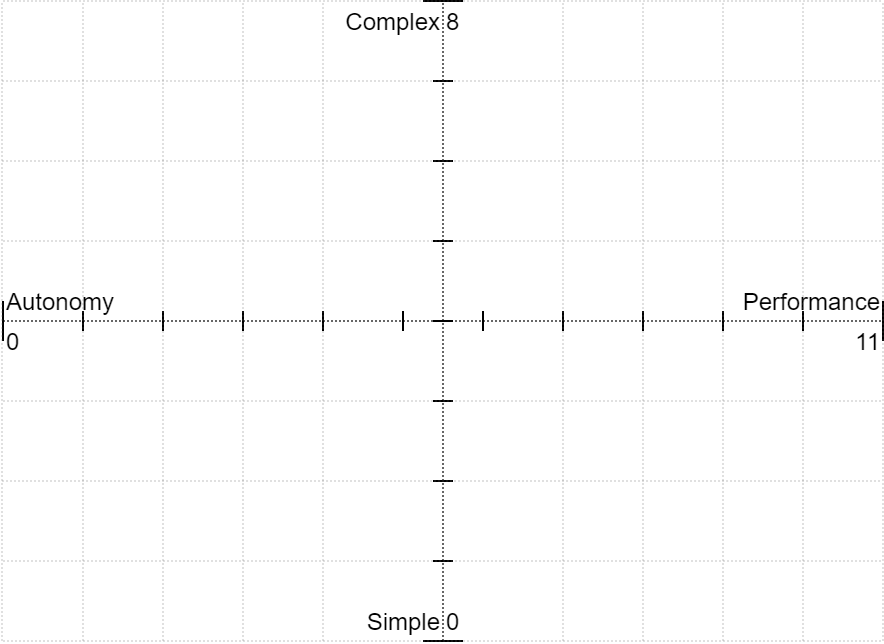
\includegraphics[scale=0.5]{quadrant_chart.png}
      \caption{Quadrant chart of the opposing questions, simplicity vs. complexity, and autonomy vs. performance}
      \label{img:quadrant_chart}
\end{figure}

The graph can be used to compare applications in one image.
It provides an overview of the driving affiliations for an application.
Both assessment Tables \ref{tbl:application_assessment} and \ref{tbl:shell_assessment} only reflect the amount of approaches taken into a certain direction, rather than actually outlining how strong an application invests into any of the directions.
Therefore, it is hard to determine the significance of this chart, but it is a first approach on providing an overview.





\subsection{Analysis conclusion}

The requirement analysis resulted in 23 requirements and many approaches.
To better outline which of the requirements are actually important, they are firstly grouped into categories.
These categories were then ordered by importance, see \ref{cha:requirement_categories}.
After that, the requirements within each categories were ordered by importance, see \ref{cha:requirements_overview}.
Finally, each requirement with their approaches are explained, which resulted in many cross-references and partially overlapping information.
Therefore, the section \ref{cha:requirements_conclusion} outlines important facts that became apparent while working on the requirement analysis.
The section \ref{cha:requirements_conclusion_assessment} is used in the next chapter to compare different applications against each other.


